The goal of this chapter is to provide a viewpoint on the previous chapter from
the perspective of categories and in turn generalize the approach, as well as
provide proofs for the general method. However this chapter also serves as background for \Cref{sect:Anyons}. In \Cref{cat:sub:introCat} we provide a
short introduction to category theory, from the perspective of quantum
parallelism, and the structures we have already met in the discussion on
representations and anyons. In \Cref{cat:sub:categoricalQuantum} we give a short
review of how familiar structures such as the no-cloning theorem arise from the
categorification of quantum mechanics. In \Cref{cat:sub:decomp} we provide the
core theory in terms of the decomposition, which is crucial to previous
chapters. Naturally, this incurs a rigorous explanation of fusion trees. 

There are numerous introductions to the theory of tensor and fusion categories,
especially in the context of anyon models. Initially proposed by
\textcite{kitaevAnyonsExactlySolved2006} based on ideas in
\textcite{reshetikhinInvariants3manifoldsLink1991}, and furhter developed in
\textcite{bondersonNonAbelianAnyonsInterferometry2007} and \cite{wangTQC}. More
detailed and modern reviews are given by \textcite{ValeraThesis}\todo{replace iwth
the publication (shared)} \textcite{Bartlett??}.

There also appears to be a difference in treatment, fist only in terms of
algebras and string algebras \textcite{simonTopologicalQuantum2023}, then in
terms of categories as purely categorical objects and then again as categoires
of temperly lieb algebras. How do all these differ in concept / what do we gain
and lose moving between them?

\section{Tensor \& Fusion Categories}\label{cat:sub:introCat}

The general idea of a category is that it admits a sort of \emph{interface}. As noticed,
there are many similarities in data and structure between the entities we already dealt
with, i.e. the tensor product of vector space, the tensor product of representations, of
Hilbert spaces etc.... We can view all these concepts as a category with additional
constraints added.

\begin{definition}\label{cat:def:category}
  A \emph{\green {category}} $\mathcal{C}$ consists of\todo{Mention consisting of data?}
  \begin{itemize}
    \item a set of \emph{objects} $\mathrm{ob}(\mathcal{C})$,
    \item for every pair $A, B \in \mathrm{ob}(\mathcal{C})$, a \emph{hom-set} $\Hom_{\mathcal{C}}(A,B)$ of \emph{morphisms} $f : A \to B$,
    \item for every $A \in \mathrm{ob}(\mathcal{C})$, an \emph{identity morphism} $\id_A : A \to A$,
    \item for every triple $A,B,C \in \mathrm{ob}(\mathcal{C})$, a \emph{composition} map
    \[
      \circ \, : \, \Hom_\CC(B,C) \times \Hom_\CC(A,B) \longrightarrow \Hom_\CC(A,C),
    \]
  \end{itemize} such that composition is \emph{associative}, i.e.\ $(f \circ g) \circ h =
  f \circ (g \circ h)$ whenever defined, and \emph{unital}, i.e.\ $f \circ \mathrm{id}_A =
  f = \mathrm{id}_B \circ f$ for all $f : A \to B$.
\end{definition}

We want to embed some of the larger structures of $\Rep(G)$ and $\VecCat{\C}$
into the categorical formalism. For fdVect, the hom spaces of linear maps $V \to
W$ have a natural identification as a vector space as well. The composition map
is $\C$-bilinear. This immedeately motivates the following definition:

\begin{definition}\label{cat:def:clinear}
  A \green{\emph{$\C$-linear category}} \todo{Check if we need enrichment.} endows each of its hom-sets with a module structure, such that the composition is bilinear. That is
  \[
    \circ \, : \, \Hom_\mathcal{C}(B,C) \times \Hom_\mathcal{C}(A,B) \longrightarrow \Hom_\mathcal{C}(A,C)
  \]
  is $\C$-bilinear: for all $f, f' : B \to C$, \,\, $g, g' : A \to B$, and $c \in \C$,
  \[
    (f + f') \circ g = f \circ g + f' \circ g, \qquad
    f \circ (g + g') = f \circ g + f \circ g', \qquad
    (cf) \circ g = c(f \circ g) = f \circ (cg).
  \]
\end{definition}

We will now explore how to use category theory to model quantum processes. We want this to
be able to do a list of things. First, given two systems $A$ and$B$, we want the combined
system to be an object as well. Given processes, i.e. operators on each individual system
$f : A \to A^\prime$,$g : B \to B^\prime $, there should be a combined process.
Additionally, structures such as entanglement and no-cloning should be readily apparent in
this theory.

\todo{Do we need to give an intro to these properties?} Consider the tensor product $\otimes_{\mathbb{C}}$ of vector spaces $V$,$W$. We can define
this using a \emph{universal property}.

This should motivate the following definition:

\begin{definition}\label{cat:def:monoidalCat}
  A \emph{\green{monoidal category}} $\CC$ is a category that admits a unit object $I \in ob(\CC)$ and a bifunctor $\otimes : \CC \times \CC \to \CC$, as well as 3 constraining isomorphisms
  \[
      \rho_A : A \otimes I \cong A \qquad \lambda_B : I \otimes B \cong B \qquad \alpha_{ABC} : (A \otimes B) \otimes C \cong A \otimes (B \otimes C)
  \]
  such that the following diagrams commute:
  \begin{center} % Is there really no way ro make this work as a tikzcd?
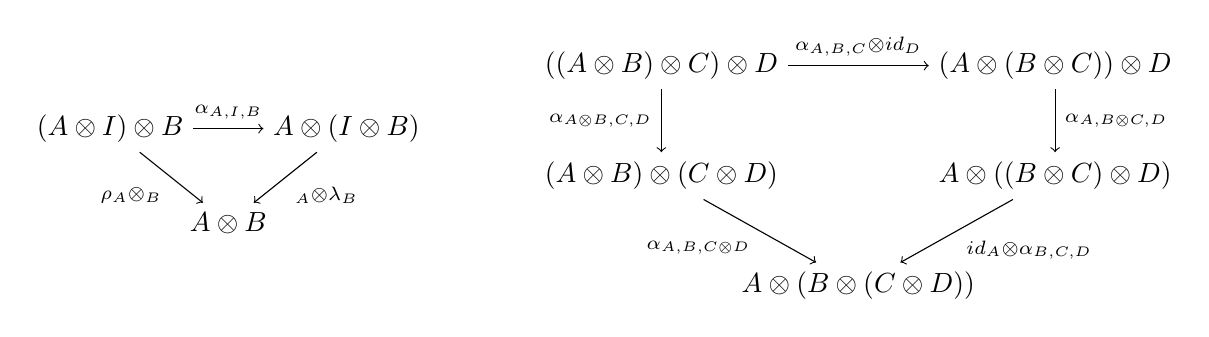
\begin{tikzpicture}[baseline=(current bounding box.center)]\label{cat:def:monoidalCat:pentagon}
  \node (AIB)  at (0,1.2)   {$(A \otimes I) \otimes B$};
  \node (AIB2) at (3,1.2)   {$A \otimes (I \otimes B)$};
  \node (AB)   at (1.5,0)     {$A \otimes B$};

  \draw[->] (AIB)  -- node[above] {$\scriptstyle \alpha_{A,I,B}$} (AIB2);
  \draw[->] (AIB)  -- node[below left]  {$\scriptstyle \rho_A \otimes \id_B$} (AB);
  \draw[->] (AIB2) -- node[below right] {$\scriptstyle \id_A \otimes \lambda_B$} (AB);
\begin{scope}[shift={(7.0,0)}]
  \node (TL) at (0,2)     {$((A \otimes B) \otimes C) \otimes D$};
  \node (TR) at (5,2)     {$(A \otimes (B \otimes C)) \otimes D$};
  \node (ML) at (0,0.6)   {$(A \otimes B) \otimes (C \otimes D)$};
  \node (MR) at (5,0.6)   {$A \otimes ((B \otimes C) \otimes D)$};
  \node (B)  at (2.5,-0.8)  {$A \otimes (B \otimes (C \otimes D))$};

  \draw[->] (TL) -- node[above] {$\scriptstyle \alpha_{A,B,C} \otimes id_D$} (TR);
  \draw[->] (TL) -- node[left]  {$\scriptstyle \alpha_{A \otimes B, C, D}$} (ML);
  \draw[->] (TR) -- node[right] {$\scriptstyle \alpha_{A, B \otimes C, D}$} (MR);
  \draw[->] (ML) -- node[below left]  {$\scriptstyle \alpha_{A,B,C \otimes D}$} (B);
  \draw[->] (MR) -- node[below right] {$\scriptstyle id_A \otimes \alpha_{B,C,D}$} (B);
\end{scope}
\end{tikzpicture}
\end{center}
For simplicity we denote a monoidal category as the sextuple $(\CC, \otimes, I, \alpha, \lambda, \rho   )$.
\end{definition}

\begin{graphicalCalculus}
  We denote the elemenets of this Category by simple lines, and the morphisms as
  boxes between these lines. Since the tensor product corresponds to paralell
  execution, we describe tensored objects as parallel lines and tensored
  operators as parallel squares.
\end{graphicalCalculus}

The commuting condition in \cref{cat:def:monoidalCat:pentagon} is an instance of
the \emph{MacLane-coherence-theorem} \cite{maclane?} (for monoidal categories). This asserts
that for any number of objects, from an initial bracketing to a final
bracketing, all morphisms must be equal.

\todo{In fact, this is important in terms of the algorithms that are used in the
reshape operation. Link here to the algorithm section. How to minimize? Can we
cache these moves?}

\begin{definition}
Let $(\mathcal{V}, \ot_\mathcal{V}, I, \alpha, \lambda, \rho)$ be a monoidal category. A category
$\CC$ \green{\emph{enriched over $\mathcal{V}$}} (or a \emph{$\mathcal{V}$-category})
consists of
\begin{enumerate}
  \item for every $A, B \in \ob(\CC)$, a \emph{hom-object} $\Hom_\CC(A,B) \in \mathcal{V}$ (as opposed to Set in normal category),
  \item for every triple $A,B,C \in \ob(\CC)$, a \emph{composition morphism} in $\mathcal{V}$
  \[
    \circ_{A,B,C} : \Hom_\CC(B,C) \ot_\mathcal{V} \Hom_\CC(A,B) \longrightarrow \Hom_\CC(A,C),
  \]
  \item for every $A \in \ob(\CC)$, a \emph{unit morphism} in $\mathcal{V}$
  \[
    j_A : I \longrightarrow \Hom_\CC(A,A),
  \]
\end{enumerate}
\end{definition}


\begin{definition}\label{cat:def:braidedMonoidalCat} A \emph{\green{braided monoidal
category}} is a monoidal category $(\mathcal{C}, \otimes, I, \alpha, \lambda, \rho)$
equipped with an additional isomorphism, the \emph{\green{braiding}}
\[
  \beta_{A,B} : A \otimes B \; \cong \; B \otimes A,
\]
on $A$ and $B$, such that the following two \emph{hexagon} diagrams
commute for all $A,B,C \in \mathcal{C}$:

\begin{center}
% https://q.uiver.app/#q=WzAsMTIsWzAsMCwiKEEgXFxvdGltZXMgQikgXFxvdGltZXMgQyJdLFsxLDAsIkEgXFxvdGltZXMoQlxcb3RpbWVzIEMpIl0sWzIsMCwiKEIgXFxvdGltZXMgQylcXG90aW1lcyBBIl0sWzAsMSwiKEJcXG90aW1lcyBBKVxcb3RpbWVzIEMiXSxbMSwxLCJCIFxcb3RpbWVzIChBIFxcb3RpbWVzIEMpIl0sWzIsMSwiQiBcXG90aW1lcyAoQyBcXG90aW1lcyBBKSJdLFszLDAsIkEgXFxvdGltZXMgKEIgXFxvdGltZXMgQykiXSxbNCwwLCIoQSBcXG90aW1lcyBCKSBcXG90aW1lcyBDIl0sWzUsMCwiQ1xcb3RpbWVzKEFcXG90aW1lcyBCKSJdLFszLDEsIkEgXFxvdGltZXMoQyBcXG90aW1lcyBCKSJdLFs0LDEsIihBIFxcb3RpbWVzIEMpXFxvdGltZXMgQiJdLFs1LDEsIihDIFxcb3RpbWVzIEEpIFxcb3RpbWVzIEIiXSxbMCwxLCJcXGFscGhhIl0sWzEsMiwiXFxiZXRhX3tBLEJcXG90aW1lcyBDfSJdLFszLDQsIlxcYWxwaGEiXSxbNCw1LCJcXGlkX0IgXFxvdGltZXNcXGJldGFfe0EsQ30iXSxbMCwzLCJcXGJldGFfe0EsQn1cXG90aW1lcyBcXGlkX0MiLDJdLFsyLDUsIlxcYWxwaGEiXSxbNiw3LCJcXGFscGhhXnstMX0iXSxbNiw5LCJcXGJldGEiLDJdLFs5LDEwLCJcXGFscGhhXnstMX0iLDJdLFs3LDgsIlxcYmV0YSJdLFs4LDExLCJcXGFscGhhXnstMX0iXSxbMTAsMTEsIlxcYmV0YSIsMl1d
\begin{tikzcd}[column sep=scriptsize]
	{(A \otimes B) \otimes C} & {A \otimes(B\otimes C)} & {(B \otimes C)\otimes A} & {A \otimes (B \otimes C)} & {(A \otimes B) \otimes C} & {C\otimes(A\otimes B)} \\
	{(B\otimes A)\otimes C} & {B \otimes (A \otimes C)} & {B \otimes (C \otimes A)} & {A \otimes(C \otimes B)} & {(A \otimes C)\otimes B} & {(C \otimes A) \otimes B}
	\arrow["\alpha", from=1-1, to=1-2]
	\arrow["{\beta_{A,B}\otimes \id_C}"', from=1-1, to=2-1]
	\arrow["{\beta_{A,B\otimes C}}", from=1-2, to=1-3]
	\arrow["\alpha", from=1-3, to=2-3]
	\arrow["{\alpha^{-1}}", from=1-4, to=1-5]
	\arrow["\beta"', from=1-4, to=2-4]
	\arrow["\beta", from=1-5, to=1-6]
	\arrow["{\alpha^{-1}}", from=1-6, to=2-6]
	\arrow["\alpha", from=2-1, to=2-2]
	\arrow["{\id_B \otimes\beta_{A,C}}", from=2-2, to=2-3]
	\arrow["{\alpha^{-1}}"', from=2-4, to=2-5]
	\arrow["\beta"', from=2-5, to=2-6]
\end{tikzcd}
\end{center}
\end{definition}

\begin{definition}
A braided monoidal category is \emph{\green{symmetric}} if $\beta_{B,A} \circ \beta_{A,B}
= \mathrm{id}_{A \otimes B}$ for all $A, B$.
\end{definition}

\begin{graphicalCalculus}
  Now the graphical calculus changes, as we need to consider whether the
  braidings defined by $\beta$ are over or under. We denote the simple braidings
  as \todo{Check for the correct definition of the ambient space here.}
\end{graphicalCalculus}

\begin{definition}\label{cat:def:directSum}
  Given a linear category $\CC$ with objects $\{A_j\}_{j=1}^N \subseteq \ob(\CC)$, an object $\bigoplus_{i=1}^n A_i \in \CC$ is
  called the \emph{\green{direct sum}} if it is equipped with the injection and projection
  map
  \[
    \iota_i : A_j \to \bigoplus A_i \quad \text{ and } \quad \pi_i : \bigoplus A_j \to A_i 
  \]
  such that
  \[
    \pi_i \circ \iota_i = \id_{A_i} \forall i \quad \text{ and } \quad \sum_{i}^{} \iota_i \pi_i = \id_{\bigoplus A_i}
  \]
\end{definition}

A great resource on semisimple categories \cite{bailieSemisimple2017}.

\begin{definition}\label{cat:def:semisimpleCategory} A \emph{\green{semisimple}}
  category\footnote{There are multiple definitions of semisimplicity and
  semisimple categories, and here we are using the definition of \emph{object
  simplicity}. A review of these definitions is given in
  \cite{bailieSemisimple2017}.} is a category in which every object $S \in
  \ob(\CC)$ decomposes as a finite direct sum 
  \begin{equation}\label{cat:eq:semisimple_decomp_1}
    S \cong \bop_i S_i, \qquad S_i \text{ simple }
  \end{equation}
  where a \emph{\green{simple}} object is an object, where for any other object
  $A$ that admits an injective \todo{this is vector space intuition, not sure if
  this works. Maybe we need to introduce monomorphism? Need to review this
  definition for general categories.} map, the object is either the $0$ morphism
  or an isomorphism to $S$ \todo{Is this just the first part of schurs lemma?}.
  If we group these simples by isomorphism, we can restate \eqref{cat:eq:semisimple_decomp_1} equivalently as
  $$
    S \cong \bop_i S_i^{\oplus n_i}
  $$
  where $n_i = \dim\Hom_\CC(S_i, S)$. Note that by our assumption of
  $\Veck$-enrichment, all the $n_i$s are finite. \todo{Erichment first.} Further
  denote the set of simple objects by $\Irr(\CC) \subseteq \ob(\CC)$.
\end{definition}

\begin{lemma}[Schur's lemma
    \cite{deutscheakademiederwissenschaftenzuberlinSitzungsberichteKoeniglichPreussischen1882}
  ]
  \label{cat:lemma:schur}
  If $A$ and $B$ are simple objects in a linear category over an algebraically
  closed field $k$ (this is always $\C$ in our case), then it holds that
  \[
    \Hom(A,B) = \begin{dcases}
      k \cdot \id_S, &\text{ if } A \cong B ;\\
      0 , &\text{ if } A \ncong B .
    \end{dcases}
  \]
  Proof \cite[Theorem~7.5]{ibortIntroductionGroupsGroupoids2019}.
\end{lemma}

Now assume that we take a semisimple category that is also monoidal. By
semisimplicity, any of the objects of the form $R_a \ot R_b$ are isomoprhic to $\bop R_c$
where $R_a,R_b, \{R_c\}$ are all simple. A simple consequence of \Cref{cat:lemma:schur} produces
\[
  \dim \Hom_\CC(R_a \ot R_b, R_c) 
  = \dim \Hom_\CC (\bop_c N^{ab}_d R_d, R_c) 
  = \dim \bop_d \Hom_\CC (R_d, R_c)^{\op N^{ab}_d} 
  \overeq{\cref{cat:lemma:schur}} \dim k^{N^{ab}_c}
\]
Call this isomorphism $\Phi: \bigoplus_{c,\mu} R_c \to R_a \otimes R_b$. Then we
can extend projection and injection maps in dependence of the tensor product by
the following diagram:
\begin{equation}\label{cat:eq:fusionprop}
% https://q.uiver.app/#q=WzAsNSxbMCwwLCJcXGJpZ29wbHVzX2MgUl9jIl0sWzIsMCwiUl9hIFxcb3RpbWVzIFJfYiJdLFswLDEsIlJfYyJdLFs0LDAsIlxcYmlnb3BsdXNfYyBSX2MiXSxbNCwxLCJSX2MiXSxbMCwxLCJcXFBoaSJdLFsyLDAsIlxcaW90YV9jIl0sWzIsMSwiXFxleGlzdHMgXFxpb3RhX3tjLFxcbXV9XnthYn0iLDJdLFsxLDMsIlxcUGhpXnstMX0iXSxbMyw0LCJcXHBpX2MiXSxbMSw0LCJcXGV4aXN0c1xccGlfe2FifV57YyxcXG11fSIsMl1d
\begin{tikzcd}
	{\bigoplus_c R_c} && {R_a \otimes R_b} && {\bigoplus_c R_c} \\
	{R_c} &&&& {R_c}
	\arrow["\Phi", from=1-1, to=1-3]
	\arrow["{\Phi^{-1}}", from=1-3, to=1-5]
	\arrow["{\exists\pi_{ab}^{c,\mu}}"', from=1-3, to=2-5]
	\arrow["{\pi_c}", from=1-5, to=2-5]
	\arrow["{\iota_c}", from=2-1, to=1-1]
	\arrow["{\exists \iota_{c,\mu}^{ab}}"', from=2-1, to=1-3]
\end{tikzcd}
\end{equation}

Furthermore, these admit similar constraints as the direct sum:
\begin{equation}
  \pi^{c,\mu}_{ab} \iota_{d,\nu}^{ab} = \pi_{c,\mu} \Phi^{-1}\Phi  \iota_{d,\nu} = \delta_{cd}\delta_{\mu\nu} \id_{R_c}
\end{equation}
and
\begin{equation}\label{cat:eq:basis_completeness}
  \sum_{c,\mu}^{} \iota_{c,\mu}^{ab} \pi^{c,\mu}_{ab} = \Phi \left(\sum_{c,\mu}^{} \iota_{c,\mu}\pi_{c,\mu}\right) \Phi^{-1} = \Phi \id_{\bigoplus R_{c}} \Phi^{-1} = \id_{R_a \otimes R_b}  
\end{equation}

We take these maps as above and claim they form a basis of the spaces $\Hom_\CC
(a \otimes b, c)$ and $\Hom_\CC (c, a \otimes b)$.

\begin{proof}
  First we show linear independence. Let $\{x_\mu\}_{1}^{N_c^{ab}}$ be a set of
  scalars and suppose that $\sum_\mu x_\mu \iota_{c,\mu}^{ab} = 0$. Observe that
  \[
    \pi_{c,\mu}^{ab} (\sum_{\mu} x_\mu \iota_{c,\mu}^{ab}) = \sum x_\mu \delta_{\mu,\nu} \id_{R_c} = x_\nu \id_{R_c}
  \]
  and since $\id_{R_c} \neq 0$ these form a linearly independent set. 

  Now let $f \in \Hom_\CC(R_c, R_a \ot R_b)$ be an arbitrary morphism. By
  \eqref{cat:eq:basis_completeness}, we can write
  \[
    f = \id_{R_a \ot R_b} \circ f = \sum_{d,\nu} \iota_{d,\nu}^{ab} (\pi^{d,\nu}_{ab} \circ f \in \Hom_\CC(R_c,R_d)) \overeq{\Cref{cat:lemma:schur}} \sum_{d,\nu} \iota_{d,\nu}^{ab} \delta_{R_c \cong R_d} \lambda_\nu \id_{R_c} = \sum_\nu \lambda_\nu \iota_{c,\nu}^{ab}
  \]
  and $f$ is an arbitrary linear combination and thus
  \[
    \text{span}_\C \left\{\iota_{d,\nu}^{ab}\right\}_{\nu = 1}^{N_{ab}^c} \cong \Hom_{\CC}(R_c, R_a \otimes R_b)
  \]
  and the statement follows dually for $\Hom_\CC(R_a \otimes R_b, R_c)$.
\end{proof}

If we look at $\Hom$ spaces of a higher order such as $\Hom_\CC(R_d, (R_a \ot
R_b) \ot R_c)$, we have to choose a bracketing of the tensor products since we
can only associate $(R_a \ot R_b) \ot R_c \cong R_a \ot (R_b \ot R_c)$. This
induces a pullback \footnote{We will later see this (or where i put it) that
this pullback can be assigned a matrix, and through semisimplicity sort of spans
the entire space. This is an instance of a lifting through the yoneda lemma,
i.e. we can define what $\alpha$ is doing by evaluating the action on finitely
many points, and extending this trhough semisimplicity to the full space.}
\[
  \alpha^\ast : \Hom_\CC(R_d, (R_a \otimes R_b \otimes R_c)) \cong \Hom_\CC(R_d, R_a \ot (R_b \ot R_c)).
\]
We can also define a basis for these extended spaces. In fact, lets generalize this to the space $\Hom_\CC(R_b, \bigotimes_{i=1}^n R_{a_i})$. Given an ONB $\iota^{}$ for the space $\Hom_\CC(R_b, \bigotimes_{i=1}^{n-1})$ we can extend it to a basis on the larger space by taking
\[
  \iota^n = (\iota^{n-1} \ot \id_{R_{a_n}}) \circ \iota_{b,\mu}^{c,a_n}
\]



If we want to use contractions between matchings legs, and overall want the
ability to take duals just like in $\FDVec{\C}$, we need both a concept of
duality and the evaluation maps. This is also the categorification of the
\emph{creation} and \emph{annihilation} maps from \Cref{sect:Anyons}. Let this
motivate the following definition:
\begin{definition}
  A monoidal category $(\CC, \otimes, 1)$ is \emph{\green{rigid}} if, for every $A \in \CC$, there exists a \emph{\green{dual object}} $A^\ast$ with the following maps:
  \[
    \ev_A : A^\ast \otimes A \to 1 \quad \text{ and } \quad \coev_A : 1 \to A \otimes A^\ast
  \]
  subject to the diagrammatic constraints
  % https://q.uiver.app/#q=WzAsOCxbMCwwLCIxIFxcb3RpbWVzIEEiXSxbMiwwLCIoQSBcXG90aW1lcyBBXlxcYXN0KSBcXG90aW1lcyBBIl0sWzAsMiwiQSBcXG90aW1lcyAxIl0sWzIsMiwiQSBcXG90aW1lcyAoQV5cXGFzdCBcXG90aW1lcyBBKSJdLFs0LDIsIjEgXFxvdGltZXMgQV5cXGFzdCJdLFs0LDAsIkFeXFxhc3RcXG90aW1lcyAxIl0sWzYsMiwiKEFeXFxhc3QgXFxvdGltZXMgQSkgXFxvdGltZXMgQV5cXGFzdCJdLFs2LDAsIkFeXFxhc3QgXFxvdGltZXMgKEEgXFxvdGltZXMgQV5cXGFzdCkiXSxbMCwxLCJcXGNvZXZfQSBcXG90aW1lcyBcXGlkX0EiXSxbMCwyLCJcXGxhbWJkYV9BIFxcY2lyYyBcXHJob19BIiwyXSxbMiwzLCJcXGlkXzEgXFxvdGltZXMgXFxldl9BIiwyXSxbMSwzLCJcXGFscGhhX3tBLEFeXFxhc3QsQX0iXSxbNCw2LCJcXGV2X0EgXFxvdGltZXNfe0FeXFxhc3R9IiwyXSxbNSw0LCJcXGxhbWJkYV97QV5cXGFzdH0gXFxjaXJjIFxccmhvX3tBXlxcYXN0fSIsMl0sWzYsNywiXFxhbHBoYV97QV5cXGFzdCxBLEFeXFxhc3R9IiwyXSxbNSw3LCJcXGlkX0EgXFxvdGltZXMgXFxjb2V2X0EiXV0=
  \[\begin{tikzcd}
	  {1 \otimes A} && {(A \otimes A^\ast) \otimes A} && {A^\ast\otimes 1} && {A^\ast \otimes (A \otimes A^\ast)} \\
	  \\
	  {A \otimes 1} && {A \otimes (A^\ast \otimes A)} && {1 \otimes A^\ast} && {(A^\ast \otimes A) \otimes A^\ast}
	  \arrow["{\coev_A \otimes \id_A}", from=1-1, to=1-3]
	  \arrow["{\lambda_A \circ \rho_A}"', from=1-1, to=3-1]
	  \arrow["{\alpha_{A,A^\ast,A}}", from=1-3, to=3-3]
	  \arrow["{\id_A \otimes \coev_A}", from=1-5, to=1-7]
	  \arrow["{\lambda_{A^\ast} \circ \rho_{A^\ast}}"', from=1-5, to=3-5]
	  \arrow["{\id_1 \otimes \ev_A}"', from=3-1, to=3-3]
	  \arrow["{\ev_A \otimes_{A^\ast}}"', from=3-5, to=3-7]
	  \arrow["{\alpha_{A^\ast,A,A^\ast}}"', from=3-7, to=1-7]
  \end{tikzcd}\]
\end{definition}

\newcommand{\Astrand}[2]{
  \draw[->, #1] (#2) -- ++(0,1);
}
\newcommand{\Adualstrand}[2]{
  \draw[<- , #1] (#2) -- ++(0,1);
}

\begin{graphicalCalculus}
  \todo{Do these need to point up or down?} Now we have to introduce this notion of duality on the level of the graphical
  calculus. We denote an object in the category by an oriented arrow, and denote
  its dual object by the reverse.
  \[
    \begin{tikzpicture}[baseline=-0.5ex]
      \Astrand{}{0,0}
      \node[right] at (0.1,0.5) {$A$};
    \end{tikzpicture}
    \qquad\qquad
    \begin{tikzpicture}[baseline=-0.5ex]
      \Adualstrand{}{0,0}
      \node[right] at (0.1,0.5) {$A^\ast$};
    \end{tikzpicture}
  \]
  Similarly the $\ev_{A}$ and $\coev_A$ maps induce a graphical menaing:
  \[
  \coev_A :
  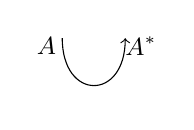
\begin{tikzpicture}[baseline=-0.5ex]
    \draw[->] (-0.4, 0.6) .. controls (-0.4, -0.2) and (0.4, -0.2) .. (0.4, 0.6);
    \node at (-0.6, 0.5) {\small $A$};
    \node at (0.6, 0.5) {\small $A^*$};
  \end{tikzpicture}
  \qquad\text{and}\qquad
  \ev_A :
  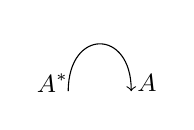
\begin{tikzpicture}
    \draw[->] (-0.4, -0.6) .. controls (-0.4, 0.2) and (0.4, 0.2) .. (0.4, -0.6);
    \node at (-0.6, -0.5) {\small $A^*$};
    \node at (0.6, -0.5) {\small $A$};
  \end{tikzpicture}.
\]

\end{graphicalCalculus}

\begin{definition}
  A \emph{\green{ribbon}} category is a braided monoidal rigid category $(\CC,\otimes,1,\alpha,\gamma,\rho,\beta,\ev,\coev)$ with maps $\theta_A : A \to A$ that realizes a \emph{self-braiding} of the object. This is subject to
  \[
    \theta_{A \otimes B} = \beta_A \beta_B \theta_A \theta_B
  \]
\end{definition}


\begin{definition}
  A $k$-enriched category $\CC$ is called semisimple if every object $X$ is ismorphic to a finite sum of simple objects. Let $\{R_a\}_a$ be representatives of the isomorphism classes of simple categories (and assume algebraic closure / absolute simplicity). 
  Then every $X$ admits as \emph{isotypic} decomposition as
  \[
    X \cong \bigoplus_{a \in L} \Hom_\CC (R_a, X) \otimes_k R_a
  \]
\end{definition}

Now we would like the category that has all of these statements combined: 

\begin{definition}
  A \green{\emph{fusion-category}} is a semisimple, $\Veck$-enriched rigid braided monoidal category, where each simple object has only \emph{finitely many} isomorphism classes. 
\end{definition}

\begin{remark}
  While each representation category $\Rep(G)$ forms a fusion category for finite $G$, this is not the case for infinite $G$ such as $\SU{2}$ or $\U{1}$. These violate the condition that there are finitely many simples. We can remedy this by instead considering a deformment of the underlying Lie-algebra as $U_q(\liesl 2)$.
\end{remark}

\subsection{Categorical Quantum Mechanics}\label{cat:sub:categoricalQuantum}

By a result of \textcite{abramskyNoCloningCategoricalQuantum2012}, building on the theory
of coecke et al., we can state the no-cloning theorem in categorical form: This asserts
that there is no diagonal $\delta : V \to  V \otimes V$ such that the following diagram
commutes: 

% https://q.uiver.app/#q=WzAsNCxbMCwwLCJWIl0sWzAsMSwiViBcXG90aW1lcyBWIl0sWzIsMCwiVyJdLFsyLDEsIlcgXFxvdGltZXMgVyJdLFswLDIsImYiXSxbMSwzLCJmIFxcb3RpbWVzIGYiXSxbMCwxLCJcXGRlbHRhIiwyXSxbMiwzLCJcXGRlbHRhIl1d
\begin{tikzcd}
  V && W \\
	{V \otimes V} && {W \otimes W}
	\arrow["f", from=1-1, to=1-3]
	\arrow["\delta"', from=1-1, to=2-1]
	\arrow["\delta", from=1-3, to=2-3]
	\arrow["{f \otimes f}", from=2-1, to=2-3]
\end{tikzcd}

\subsection{Tensor \& Fusion Categories}

\section{Decompositions for Categorical Networks}\label{cat:sub:decomp}

This chapter generalizes the decomposition in
\cite[Equation~27]{singhTensorNetworkStates2012a} to both Fusion Categories and the
Representation categories of compact groups. Note that in
\cite{devosTensorKitjlJuliaPackage2025}, such a generalization is given for
representations of finite groups, which does not include $SU(2)$. However I do not yet
know if we should do so, since I not yet sure how to argue the F moves here. If we instead
take the deformation $U_q(sl_2)$ we get finiteness (and fusion cats?), unfortunately
$U_q(sl_2)$ is not a group.





%\section{Symmetries}
%
%
%
%What do we know now? First of all, we take a symmetry group $G$ that is finite and compact (why?)[For compact groups, representations are completely reducible (Maschke) and the irreps are finite aswell. Finite groups are contained in compact groups.]. Then we look for its unitary representation $U(G)$ on a Hilbert space $H$. Furhtermore, if this is a multiparty hilbert space, lets say $n$ sites, we view the unitary representations $U_{n}$ at site $n$. The unitary representation $U_{n} : G \to Hom(V_{n} ,V_{n} )$ is a covariant linear unitary map. A map $V_{i} \to V_{j}$ is symmetric if it is an intertwiner of the representations, i.e. the following diagram commutes:
%% https://q.uiver.app/#q=WzAsNCxbMCwwLCJWX2kiXSxbMCwxLCJWX2oiXSxbMSwwLCJWX2kiXSxbMSwxLCJWX2oiXSxbMCwxLCJmIiwyXSxbMCwyLCJVX3tWX2l9KGcpIl0sWzEsMywiVV97Vl9qfShnKSIsMl0sWzIsMywiZiJdXQ==
%\[\begin{tikzcd}
%	{V_i} & {V_i} \\
%	{V_j} & {V_j}
%	\arrow["{U_{V_i}(g)}", from=1-1, to=1-2]
%	\arrow["f"', from=1-1, to=2-1]
%	\arrow["f", from=1-2, to=2-2]
%	\arrow["{U_{V_j}(g)}"', from=2-1, to=2-2]
%\end{tikzcd}\]
%Note that here $V_{i}$ is called a \emph{symmetry space}.
%
%Some examples of these groups include $\U{1}, \SU 2, \mathbb{Z}_{n}$
%
%Now where the intutitionAdiabatic nature of topological quantum gate is more shaky: Consider a symmetry space $V_i$ on a single site (why single). Then we get that it decomposes into a direct sum of irreps $V_{i}^a$,
%\[
%  V_{i}  = \bigoplus_a \bigoplus_{i = 1}^{d_{a} } V_{i}^a
%\]
%and we can easily construct an isomporphism (but this depends on choosing a basis for $D_{a}$.)
%\[
%  V_{i}  = \bigoplus_a \bigoplus_{i = 1}^{d_{a} } V_{i}^a = \bigoplus_{a} (D_{a} \otimes V_{i}^a ).
%\]
%
%Well, the isom we can construct here would look like $\bigoplus_1^{d_{a} } V_{i}^a \to D_{a} \otimes V_{i}^a$.
%
%Consider a single site of $3$ spin $1 / 2$ particles. Under $\SU 2$ this decomposes as 
%\[
%  2 \otimes 2 \otimes 2 = 4 \oplus 2 \oplus 2
%\]
%Now consider that $C^2$ is just the fundamental representation of $\SU 2$.
%
%
%Note here, an invariant subspace $W \subseteq V$ is a subset of vectors s.t. for all $U \in \SU 2$, $Uw \in W$.
%
%symmetry obviously implies pullthrough properties, do Intertwiners as well?
%
%Yes, because $U_(V \otimes W) : g \to U_V(g) \otimes U_W(g)$ and the following diagram commutes:
%
%% https://q.uiver.app/#q=WzAsNCxbMCwwLCJWX2kgXFxvdGltZXMgVl9qIl0sWzAsMSwiVl9rIl0sWzIsMSwiVl9rIl0sWzIsMCwiVl9pIFxcb3RpbWVzIFZfaiJdLFswLDEsIlQiLDJdLFsxLDIsIlVfe1Zfa30oZykiLDJdLFswLDMsIlVfe1ZfaSBcXG90aW1lcyBWX2p9KGcpIl0sWzMsMiwiVCJdXQ==
%\[\begin{tikzcd}
%	{V_i \otimes V_j} && {V_i \otimes V_j} \\
%	{V_k} && {V_k}
%	\arrow["{U_{V_i \otimes V_j}(g)}", from=1-1, to=1-3]
%	\arrow["T"', from=1-1, to=2-1]
%	\arrow["T", from=1-3, to=2-3]
%	\arrow["{U_{V_k}(g)}"', from=2-1, to=2-3]
%\end{tikzcd}\]
%
%\subsection{Some Symmetry Groups}
%
%\subsubsection{$\mathbb{Z}_n$ }
%
%This group is given by integers $0, \ldots n-1$ with addition mod $n$. Since this happens to be abelian, all the irreps are $1$ dimensional, i.e. 
%$U_a(g) : g \to Hom(\mathbb{C},\mathbb{C})$ with representatives $U_a(g) = z \mapsto e^{2\pi i a g / N} z$. What isthe fusion rule here?
%\[
%  a \otimes b \equiv (c : = a + b \mod n)
%\]
%This also does not have fusion multiplicities.
%
%\subsubsection{The group $\SU{2}$}
%
%Summarize the results from the paper here.
%
%\subsubsection{The group $\SU{2}_3$}
%
%Technically this is a fusion category, the thesis \cite{dissertation} handles this distinction. But if we think of this in terms of the programming guide, this seems to be doable using a group.
%
%Now, since we can argue that Products of symmetry groups again form a symmetry group (proof?), we would also need another type for sector.
%
%We could use $class Sector(NamedTuple)$ holding an array charges.
%
%\subsection{Notes on structural tensors and fusion trees}
%
%What do the CG tensors look like? As they are three index and have no intermediates, these are simply $Q_{j_1,j_2,j_3} = (C^{fuse})_{(j_1,m_{j_1}), (j_2, m_{j_2})}^{(j_3,m_{j_3})}$.
%
%\subsection{Notes on the papers}
%
%Lets assume we only look at incoming legs, i.e. we look at $T_{j_{a} ,j_{b} , j_{c} }$ in a composite vectors space $V^a \otimes V^b \otimes V^c$. By the decomposition
%\[
%  V^a \otimes V^b \otimes V^c = \left(\bigoplus_{j_a} D_{j_{a} } \otimes V_{j_{a} } \right) \otimes \left(\bigoplus_{j_b} D_{j_{b} } \otimes V_{j_{b} } \right) \otimes\left(\bigoplus_{j_c} D_{j_{c} } \otimes V_{j_{c} } \right)
%\]
%and we can represent a single index inside the block space 
%\[
%  T_{j_{a} ,j_{b} , j_{c} } \in (D_{j_{a} j_{b} j_{c}} \otimes V_{j_{a} j_{b} j_{c} })
%\]
%Choosning a basis $t = (t_{j_{a} }, t_{j_{b} }, t_{j_{c} })$ and $m = (m_{j_{a} }, m_{j_{b} }, m_{j_{c} })$ we can write
%\[
%  T_{j_a, j_b,j_c} = \sum_{t,n}^{} (T_{j_{a} ,j_{b} ,j_{c} })_{t,m} (\ket{t} \otimes \ket m)
%\]
%Now we can use Wigner-Eckart to obtain
%\[
%  T_{j_a, j_b,j_c} = \sum_{t,n}^{} ((P_{j_{a} j_{b} j_{c} })_t \cdot (Q_{j_{a} j_{b} j_{c} })_m)_{t,m} (\ket{t} \otimes \ket m)
%\]
%\[
%  = \left(\sum_{t}^{} (P_{j_{a} j_{b} j_{c} })_t \ket t\right) \otimes \left(\sum_{m}^{} (Q_{j_{a} j_{b} j_{c} })_m \ket m \right) = P_{j_{a} j_{b} j_{c} } \otimes Q_{j_{a} j_{b} j_{c} }
%\]
%
%If we generalize this with the decomposition for $k$ indices $i = (i_1, i_2, \ldots, i_k)$ and let $j_e = (j_{e_1}, j_{e_2}, \ldots, j_{e_{k-3} })$ be the internals
%\[
%  T_{i} = \sum_{j_e} (P_j^{j_e})_t \cdot (Q_j^{j_e})_m 
%\]


\begin{lemma}[Isotypic Decomposition]
\label{lem:IsotypicDecomposition}
Let $\CC$ be a $k$-enriched semisimple category and $V \in \Veck$. We now give the concept of a \emph{\green{degeneracy space}}, where we give a ??? notion of the n-fold direct sum:
\[
  V \kot R_a \cong R_a^{\op \dim{V}}
\]
How do we make this canonical? by choosing $V = \Hom_{\CC}(R_a, V)$.
\end{lemma}



\begin{lemma}
  \label{lem:IsotopyHelper}
  For a vector space $W$, there is an isomorphism
  \[
    \bigoplus^m W \simeq \mathbb{C}^m \otimes W.
  \]
\end{lemma}
\begin{proof}
  Let ${e_i}_{i \in [m]}$ be the standard basis on $\mathbb{C}^m$. Let
  \[
    \Phi : \mathbb{C}^m \otimes W \to \oplus^m W
  \]
  be defined by
  \[
    \phi(e_i \otimes w) = (0, \ldots , w, \ldots 0  )
  \]
  and linear, thus
  \[
    \Phi\left(\sum_{i}^{} c_{i} e_{i} \otimes w_{i} \right) = (c_1 w_1, \ldots , c_m w_m ).
  \]
  is clearly bijective, and we have our desired isomorphism.
\end{proof}

\begin{lemma}
  Let $D$ be a finite dimensional $k$-vector space and let $V$ be an object of a
  $k$-linear category $C$. Then
  \[
    D \otimes V
    \cong
    V^{\oplus \dim D}
  \]
\end{lemma}
\begin{proof}
  Let $n = \dim D$. Take a basis $\{e_i\}$ for D. This yields an isomorphism
  \[
    D \cong \bigoplus_{i=1}^n k \cdot e_{i} \cong k^n
  \]
  Since in a $k$-linear category the tensor product is additive (should we prove this?),
  we can distribute
  \[
    D \otimes W \cong \bigoplus_1^n (k \cdot e_{i} \otimes W) \cong \bigoplus W = W^{\oplus n}
  \]
\end{proof}

\begin{lemma}[Isotopic Decomposition]
  \label{IsotopicDecomposition}
  Let $C$ be a semisimple $k$-linear category with simple objects $\{R_a\}$. Then every
  object $V \in C$ admits a canonical decomposition
  \begin{equation}
    V \cong \bigoplus_a D_a \otimes R_{a}.
  \end{equation}
  where we refer to $D_a \coloneqq \Hom_C(R_a, V)$ as the \emph{degeneracy} of the space.
\end{lemma}

\begin{proof}
  Since $C$ is semisimple, there exist integers $m_a\ge 0$ such that
  \[
    V
    \cong
    \bigoplus_{a \in L} \bigoplus_{\_ = 1}^{D_a^V} a
    \cong
    \bigoplus_{a\in L} R_a^{\oplus m_a}.
  \]

  Applying the additive functor $\Hom_C(R_b,-)$ yields
  \[
    \Hom_C(R_b,V)
    \cong
    \bigoplus_{a\in L} \Hom_C(R_b,R_a^{\oplus m_a}) \cong \bigoplus_{a\in L} \Hom_C(R_b,R_a)^{\oplus m_a}.
  \]

  Then, by Schurs lemma
  \[
    \bigoplus_{a \in L} Hom_C(R_b, R_a)^{\oplus m_a} = k^{\oplus m_b}
  \]

  %Since $C$ is additive,
  %\[
  %  \Hom_C(R_b,V)
  %  \cong
  %  \bigoplus_{a\in L} \Hom_C(R_b,R_a)^{\oplus m_a}.
  %\]
%
%  Since $C$ is semisimple, every object decomposes as
%  \[
%    V \equiv \bigoplus_a m_a R_a
%  \]
%  for the degeneracies $m_a \in N$ (this is techinically abuse of notation, if we define the direct sum.)
%
%  Applying $Hom(R_a, -)$ (this is a linear functor?) yields
%  \[
%    Hom(R_b, V) \cong \bigoplus_a Hom(R_b, m_a R_a) \cong Hom_C(R_b, R_a)^{\oplus m_a}
%  \]
%  and then by Schur's lemma
%  \[
%    Hom_C(R_a,R_b) = \begin{dcases}
%      \mathbb{C}, &\text{ if } a \equiv b ;\\
%      0 &\text{ otherwise } 
%    \end{dcases}
%  \]
%  and therefore $dim Hom_C(R_a, V) = dim \mathbb{C}^{m_{a}} = m_a$.
%
%  An issue here might be that $Hom_C(R_a, V)$ is not an object or a morphism of $Rep(G)$. Its elements are, but not itself, it is in $Vect$.
\end{proof}

So we actualy need this: Maybe this is simpler if we always let the degeneracy be $C$?
\begin{lemma}\label{HomTensorFactorization}
Let $C$ be a $k$-linear category and let $D,E$ be finite-dimensional
$k$-vector spaces. For any objects $R,S\in C$, there is a natural
isomorphism
\[
\Hom_C(D\otimes R,E\otimes S)
\cong
\Hom_k(D,E)\otimes \Hom_C(R,S).
\]
\end{lemma}

\begin{proof}
Let $m=\dim_k D$ and $n=\dim_k E$. Proof by isomorphism chains:
$$
  \begin{aligned}
    \Hom_C(D\otimes R,E\otimes S)
    &\cong \Hom_C(R^{\oplus m},S^{\oplus n})
    && \text{by \cref{lem:IsotopyHelper}} \\[1ex]
    &\cong \bigoplus_{i=1}^{m} \bigoplus_{j=1}^{n} \Hom_C(R,S)
    && \text{by additivity of $\Hom_C$} \\[1ex]
    &\cong k^{mn} \otimes \Hom_C(R,S)
    && \text{by \cref{lem:IsotopyHelper}} \\[1ex]
    &\cong \Hom_k(D,E)\otimes \Hom_C(R,S)
    && \text{since $\Hom_k(D,E) \cong k^{mn}$}
  \end{aligned}
$$
(The last as s)
\end{proof}

\begin{definition}[Copower]
  For a $\Veck$-enriched (and tensored?) category $\mathrm{C} $, and $E \in \Veck, X \in C$ the power $X^E$ is the object of $C$ representing the natural isomorphism
  \[
    \Hom_C(Y,X^E) \cong \Hom_k(E, \Hom_C(Y,X))
  \]
\end{definition}

\begin{theorem}[Decomposition of Semisimple Categories]
  \label{DecompositionOfSemisimpleCategories}
  Let $C$ be a semisimple, monoidal, $k$-linear category whose tensor product is
  $k$-linear in each variable, with simple objects $\{R_a\}_{a\in L}$ and let $V_i, W_i$
  be a collection of (not necessarily simple) objects in $C$. Every morphism
  \[
    T \in \Hom_C\left(\bigot_{i = 1}^n V_i, \bigot_{i = 1}^m W_{i}\right)
  \]
  admit a decomposition as
  \[
    T \cong \bop_{\hat a,\hat b}
    \Hom_{k}(D_{\hat a}, E_{\hat b}) \ot_k \Hom_C(R_{\hat a},R_{\hat b}),
  \]
  where $\hat a = (a_1, \ldots , a_n )$ and $P$ is a $k$-vector space of dimension ???
\end{theorem}

\begin{proof}
\begin{align*}
\Hom_C&\!\left(
  \bigot_i V_i,
  \bigot_j W_j
\right) \\
&\cong
\Hom_C\!\left(
  \bigot_i
  \Bigl(
    \bop_{a_i}
    D_{i,a_i}\ot R_{a_i}
  \Bigr),
  \,
  \bigot_j
  \Bigl(
    \bop_{b_j}
    E_{j,b_j}\ot R_{b_j}
  \Bigr)
\right)
&\text{(\textcolor{gray}{\Cref{IsotopicDecomposition}})} 
\\[1.5ex]
&\cong
\Hom_C\!\left(
  \bop_{\hat a}
  D_{\hat a}\ot R_{\hat a},
  \,
  \bop_{\hat b}
  E_{\hat b}\ot R_{\hat b}
\right)
&\text{(\textcolor{gray}{linearity of $\ot$})}
\\[1.5ex]
&\cong
\bop_{\hat a,\hat b}
\Hom_C\!\left(
  D_{\hat a}\ot R_{\hat a},
  E_{\hat b}\ot R_{\hat b}
\right)
&
\text{\textcolor{gray}{(additivity of $\Hom_{\CC}$)}} 
\\[1.5ex]
&\cong
\bigoplus_{\hat a,\hat b}
\Hom\!\left(
  D_{\hat a},
  E_{\hat b}
\right)
\otimes
\Hom_C\!\left(
  R_{\hat a},
  R_{\hat b}
\right)
&\text{\textcolor{gray}{(\Cref{HomTensorFactorization})}} 
\end{align*}
In a basis expansion this then looks like
\[
  \cong
\bigoplus_{\hat a,\hat b}
\sum_{e,f,\mu,\nu}
\Hom\!\left(
  D_{\hat a},
  E_{\hat b}
\right)
\otimes_k
\mathsf{T}^{\widehat a,\widehat b}_{e,f;\mu,\nu}
\]
\end{proof}

\begin{corollary}[Operators are block matrices
\cite{kongInvitationTopologicalOrders2022b}] % TODO figure out why i cant cie theorems in
thm header.
  \label{cor:operator_blocks}
  An operator
  \[
    Hom(V,W) 
    \cong
    Hom_C\bigl(\bigoplus_a R_a^{\oplus d_a}, \bigoplus_b R_b^{\oplus e_b} \bigr) \cong \bigoplus_{a,b} Hom(D_a, E_b) \otimes Hom_C(R_a, R_b)
  \]
  and by Schurs lemma this is just
  \[
    \bigoplus_{a \in Irr(V) \cap Irr(W)} Hom(D_a, E_a) \cong \bigoplus_{a \in Irr(V) \cap Irr(W)} Mat_{d_a \times e_a}(k)
  \]
\end{corollary}

\begin{corollary}
  Let $Q_{\mu, \eta}$ be a basis of $Hom_C\bigl(\bigotimes_{\hat{a}} R_{\hat{a}},
  \bigotimes_{\hat{b} } R_{\hat{b} }  \bigr)$ where $\mu$ denotes the multiplicities and
  $\eta$ the internal fusions. In a \emph{multiplicity-free} Category we will omit $\mu$
  as a label. 
\end{corollary}

\begin{example}
  However, now assign $V_{\frac{1}{2}} \otimes V_{\frac{1}{2}}$ to each leg in the example
  above. Each leg then becomes $V_0 \oplus V_1 \cong \mathbb{C} \otimes V_0 \oplus
  \mathbb{C} \otimes V_1$. Then we can start with the decomposition.
  \[
    Hom_C(\bigoplus_{a,b,c \in (0,1)} (C \otimes C \otimes C) \otimes V_a \otimes V_b \otimes V_c, \bigoplus_{b \in (0,1)} C \otimes V_b) 
  \]
  \[
    = \bigoplus_{a,b,c,d \in (0,1)} Hom_C((C \otimes C \otimes C) \otimes (V_a \otimes V_b \otimes V_c), C \otimes V_d)
  \]
  \[
    = \bigoplus_{a,b,c,d} Hom(C^3, C) \otimes Hom_{\Rep(SU(2))} (V_a \otimes V_b \otimes V_c, V_d)
  \]
\end{example}

\begin{example}
  Easier. However, now assign $V_{\frac{1}{2}} \otimes V_{\frac{1}{2}}$ to each leg in the
  example above. Each leg then becomes $V_0 \oplus V_1 \cong \mathbb{C} \otimes V_0 \oplus
  \mathbb{C} \otimes V_1$. Then we can start with the decomposition.
  \[
    Hom_C\left(\bigoplus_{a,b\in (0,1)} (C \otimes C) \otimes V_a \otimes V_b \bigoplus_{b \in (0,1)} C \otimes V_b \right) 
  \]
  \[
    = \bigoplus_{a,b,c \in (0,1)} Hom_C((C \otimes C) \otimes (V_a \otimes V_b), C \otimes V_c)
  \]
  \[
    = \bigoplus_{a,b, c} Hom(C^2, C) \otimes Hom_{\Rep(SU(2))} (V_a \otimes V_b, V_c)
  \]
\end{example}


\begin{example}
  Lets look at a tensor with in legs $(\tau \otimes \tau)$ and $\tau$ and out legs $\tau$.
  \[
    Hom_C(((k \otimes 1) \oplus (k \otimes \tau)) \otimes (k \otimes \tau), k\otimes\tau)
    =
    Hom_C()
  \]
  \[
    \begin{aligned}
      &\Hom_C\bigl(((k \otimes 1) \oplus (k \otimes \tau)) \otimes (k \otimes \tau),\, k\otimes\tau\bigr)\\
      &\cong
      \Hom_C\bigl((k\otimes1\otimes k\otimes\tau)
      \oplus
      (k\otimes\tau\otimes k\otimes\tau),\,k\otimes\tau\bigr)\\
      &\cong
      \Hom_C(k\otimes 1 \otimes k \otimes\tau,\,k\otimes\tau)
      \oplus
      \Hom_C(k\otimes \tau \otimes(k \otimes\tau),\,k\otimes\tau)\\
      &\cong
      \Hom(k \otimes k,k)\otimes\Hom_C(1 \otimes \tau,\tau)
      \oplus
      \Hom(k \otimes k,k)\otimes\Hom_C(\tau\otimes\tau,\tau).
    \end{aligned}
  \]
\end{example}

\begin{example}[Anyonic matrix operator]
  Finally, consider a $4 \to 4$ anyon operator with one leg on each side, representing the
  space $\mathrm{Hom}((\tau \otimes \tau \otimes \tau \otimes \tau), (\tau \otimes \tau
  \otimes \tau \otimes \tau))$. THe full decomposition is $2 + 3\tau$. Hence we obtain
  \[
    \Hom_C\!\left(
      (k^2 \otimes 1)\oplus(k^3\otimes\tau),
      (k^2 \otimes 1)\oplus(k^3\otimes\tau)
    \right).
  \]
  \[
    =
    \bigoplus_{a,b\in(1,\tau)}
    \Hom_C(k^{m_a}\otimes a,\,
    k^{m_b}\otimes b)
    =
    \bigoplus_{a,b\in(1,\tau)}
    \Hom(k^{m_a}, k^{m_b}) \otimes Hom_C(a,b)
  \]
  where
  \[
    m_1=2,
    \qquad
    m_\tau=3.
  \]
  For this case, Schurs lemma applies. So we have
  \[
    = Hom(k^2, k^2) \oplus Hom(k^3, k^3)
  \]
  which is just a block matrix with indexing $(1_1, 1_2, \tau_1, \tau_2, \tau_3)$.
\end{example}

\begin{example}[$U(1)$ Symmetry]
  Technically we would want to show here that this is simpler in general. TOOD. Make a theorem? Or a corollary?
\end{example}


\begin{equation}
  \label{ExternalTensorProductAsCoproductOfFiberwiseTensor}
  \begin{aligned}
    \mathscr{V}_X \boxtimes \mathscr{V}'_{X'}
    &\simeq \Bigl(\, \coprod_{x \in X} \mathscr{V}_{\{x\}} \Big) \boxtimes \Big(\, \coprod_{x' \in X'} \mathscr{V}'_{\{x'\}} \Big)
    && \text{by \eqref{VectorBundleOverSetIsCoproductOfItsRestrictionToSingletons}} \\[1ex]
    &\simeq \coprod_{x \in X} \bigg(\!\! \mathscr{V}_{\{x\}} \boxtimes \Big(\, \coprod_{x' \in X'} \mathscr{V}'_{\{x'\}} \Big) \!\! \bigg)
    && \text{by assumption (i) in first variable} \\[1ex]
    &\simeq \coprod_{x \in X} \; \coprod_{x' \in X'} \Big( \mathscr{V}_{\{x\}} \boxtimes \mathscr{V}'_{\{x'\}} \Big)
    && \text{by assumption (i) in second variable} \\[1ex]
    &\simeq \coprod_{x \in X} \; \coprod_{x' \in X'} \Big( \iota \big( \mathscr{V}_x \otimes \mathscr{V}_{x'} \big) \Big)
    && \text{by assumption (ii)} \\[1ex]
    &\simeq \coprod_{(x,x') \,\in\, X \times X'} \Big( \iota \big( \mathscr{V}_x \otimes \mathscr{V}_{x'} \big) \!\Big)
    && \text{just to make the base space manifest}
  \end{aligned}
\end{equation}

\subsection{Algorithms for contracting dual networks}

\section{Tensor and Fusion Categories}


Let $C$ and $D$ be linear abelian categories. Then the \emph{Deligne Tensor Product} $C \boxtimes D$ is a linear abelian category with a bifunctor
\[
  \boxtimes : C \times D \to C \boxtimes D
\]
with morphisms given by
\[
  Hom_{C \boxtimes D}(X \boxtimes Y, W \boxtimes V) = Hom_C(X,W) \otimes Hom_D(Y,V)
\]

\begin{definition}[The Deligne Tensor Product of Categories]
Let $k$ be a field, and let $\mathcal{C}$ and $\mathcal{D}$ be two $k$-linear, finite abelian categories. The \textbf{Deligne tensor product}, denoted by $\mathcal{C} \boxtimes \mathcal{D}$, is a $k$-linear finite abelian category equipped with a $k$-bilinear functor
\[ \boxtimes: \mathcal{C} \times \mathcal{D} \longrightarrow \mathcal{C} \boxtimes \mathcal{D}, \quad (X, Y) \mapsto X \boxtimes Y \]
TODOTOD!!
\end{definition}


\begin{definition}[The Category $\Rep_k(G)$]
  Let $G$ be a group and $k$ a field. The \emph{category of linear representations of $G$ over $k$} consists of the following data:

  \begin{itemize}
    \item \textbf{Objects:} The objects $\Rep_k(G)$ are pairs $(V, \rho_V)$, where $V$ is a $k$-vector space and $\rho_V : G  \to \mathrm{GL}(V)$.  
    \item \textbf{Morphisms:} For any two objects $(V, \rho_V)$ and $(W, \rho_W)$ in $\Rep_k(G)$, a morphism from $V$ to $W$ is a $k$-linear transformation $f: V \to W$ that is $G$-invariant (also called an \textit{intertwiner}). That is, for every element $g \in G$, the following diagram commutes:
    \[
    \begin{tikzcd}
    V \arrow[r, "\rho_V(g)"] \arrow[d, "f"'] & V \arrow[d, "f"] \\
    W \arrow[r, "\rho_W(g)"']               & W
    \end{tikzcd}
    \]
    In algebraic terms, $f$ must satisfy the condition:
    \[ f \circ \rho_V(g) = \rho_W(g) \circ f \quad \forall g \in G \]
    The set of all such morphisms is denoted by $\mathrm{Hom}_G(V, W)$.
  \end{itemize}
  We can further endow $Rep_k(G)$ with a monoidal structure: For any two objects $(V,\rho_V), (W,\rho_W)$, their tensor product is in $\Rep_k(G)$ by the diagonal action
  \[
    \rho_{(V \otimes W)} (g) (v \otimes w) = \rho_V(g)v \otimes \rho_W(g)w
  \]
\end{definition}



\begin{theorem}[Fusion Representation Category of finite groups]
  \label{thm:finiteGroupFusionCat}
  Let $G$ be a finite group. Then $\Rep(G)$ is a fusion category.
\end{theorem}

\begin{theorem}
  Let $G_1$ and $G_2$ be finite groups and let $\Rep(G_1), \Rep(G_2)$ be their respective symmetry categories. Then there is an equivalence of categories
  \[
    \Rep(G_1 \times G_2) \simeq \Rep(G_1) \boxtimes \Rep(G_2)
  \]
\end{theorem}





Lets give a coordinatized approach to fusion categories:

\begin{definition}[Fusion Category in Vector Form]
  A \emph{fusion category} is a finite set of labels (sectors?) $L$ and vector spaces $V^{ab}_c$ for all $a,b,c \in L$, as well as the isomorphisms
  \[
    F^{abc}_{d} : \bigoplus_e V^{ab}_e \otimes V^{ec}_d \to \bigoplus_e V^{ae}_d \otimes V^{bc}_e
  \]
  such that the pentagon holds.
\end{definition}


\begin{equation}
\text{Hom}\left( \bigotimes_{k=1}^m X_{i_k}, \bigotimes_{l=1}^n X_{j_l} \right) = \text{span}_{\mathbb{C}} \left\{
\begin{gathered}
\begin{tikzpicture}[
    baseline=(current bounding box.center),
    scale=1.2,
    string arrow/.style={
        postaction={decorate},
        decoration={
            markings,
            mark=at position 0.55 with {\arrow[scale=1.0]{Stealth}}
        }
    }
]
    % Boundary Input Nodes
    \node (xi1) at (-3.4, 3.2) [above] {$X_{i_1}$}; % I dont get why it is assym with -3.2
    \node (xi2) at (-2.5, 3.2) [above] {$X_{i_2}$};
    \node (xi3) at (-1.8, 3.2) [above] {$X_{i_3}$};
    \node at (-0.5, 3.2) {$\cdots$};
    \node (xim1) at (0.8, 3.2) [above] {$X_{i_{m-1}}$};
    \node (xim) at (1.6, 3.2) [above] {$X_{i_m}$};

    % Internal Vertices
    \coordinate (Ve1) at (-2.7, 2.5);
    \coordinate (Ve2) at (-2.2, 1.9);
    \coordinate (Vem3) at (-1.0, 0.9);
    \coordinate (Vem2) at (-0.5, 0.4);
    \coordinate (Btop) at (0, 0.05);

    % Incoming Leaves to Vertices
    \draw[string arrow] (xi1) -- (Ve1);
    \draw[string arrow] (xi2) -- (Ve1);
    \draw[string arrow] (xi3) -- (Ve2);
    \draw[string arrow] (xim1) -- (Vem2);
    \draw[string arrow] (xim) -- (Btop);

    % Main Trunk Segments (Top)
    \draw[string arrow] (Ve1) -- (Ve2) node[below left, pos=0.4] {$e_1$};
    \draw[string arrow] (Ve2) -- (-1.9, 1.55) node[below left, pos=0.4] {$e_2$};
    
    % Diagonal Dots (Top Trunk)
    \fill (-1.65, 1.35) circle (0.8pt);
    \fill (-1.50, 1.20) circle (0.8pt);
    \fill (-1.35, 1.05) circle (0.8pt);
    
    %\draw[string arrow] (-1.2, 0.9) -- (Vem3); 
    \draw[string arrow] (Vem3) -- (Vem2) node[below left, pos=0.4] {$e_{m-3}$};
    \draw[string arrow] (Vem2) -- (Btop) node[below left, pos=0.4] {$e_{m-2}$};


    \coordinate (Bbot) at (0, -0.65);
    \draw[string arrow] (Btop) -- (Bbot) node[right, pos=0.5] {$b$};


    % Internal Vertices
    \coordinate (Vfn2) at (-0.5, -1.0);
    \coordinate (Vfn3) at (-1.0, -1.5);
    \coordinate (Vf2) at (-2.2, -2.5);
    \coordinate (Vf1) at (-2.7, -3.1);

    % Main Trunk Segments (Bottom)
    \draw[string arrow] (Bbot) -- (Vfn2) node[left, pos=0.6] {$f_{n-2}$};
    \draw[string arrow] (Vfn2) -- (Vfn3) node[left, pos=0.6] {$f_{n-3}$};
    
    % Diagonal Dots (Bottom Trunk)
    \fill (-1.35, -1.65) circle (0.8pt);
    \fill (-1.50, -1.80) circle (0.8pt);
    \fill (-1.65, -1.95) circle (0.8pt);
    
    \draw[string arrow] (-1.9, -2.15) -- (Vf2);
    \draw[string arrow] (Vf2) -- (Vf1) node[left, pos=0.4] {$f_1$};
    \path (Vf2) -- (Vf1) node[left, pos=1.2] {$f_2$}; % Label position adjustment

    % Outgoing Leaves to Boundary
    \draw[string arrow] (Vf1) -- (-3.2, -3.8);
    \draw[string arrow] (Vf1) -- (-2.5, -3.8);
    \draw[string arrow] (Vf2) -- (-1.8, -3.8);
    \draw[string arrow] (Vfn2) -- (0.8, -3.8);
    \draw[string arrow] (Bbot) -- (1.6, -3.8);

    % Boundary Output Nodes
    \node (xj1) at (-3.2, -3.8) [below] {$X_{j_1}$};
    \node (xj2) at (-2.5, -3.8) [below] {$X_{j_2}$};
    \node (xj3) at (-1.8, -3.8) [below] {$X_{j_3}$};
    \node at (-0.5, -3.8) {$\cdots$};
    \node (xjn1) at (0.8, -3.8) [below] {$X_{j_{n-1}}$};
    \node (xjn) at (1.6, -3.8) [below] {$X_{j_n}$};

\end{tikzpicture}
\end{gathered}
\right\}_{ \substack{b, \, e_1, \dots,  e_{m-2}, \, f_1, \, \dots, \, f_{n-2} \\ \mu_1, \, \dots, \, \mu_{m-2}, \, \nu_1, \, \dots, \, \nu_{n-2}} }
\end{equation}

\begin{equation}
\begin{gathered} % From the seminar paper and
\begin{tikzpicture}
  \node at (0,-0.1) {$\underset{e,f}{\bigoplus} V^{ab}_e \otimes V^{ec}_f \otimes V^{fd}_g $};
  \draw[->, black] plot coordinates{(0.4,0.5) (2.5,1.5)};
  \node at (0.9,1.3) {$id_{V_{e}^{ab}} \otimes F^{ecd}_{g}$};
  \node at (4.0,1.9)  {$\underset{e,l}{\bigoplus} V^{ab}_e \otimes V^{cd}_{f} \otimes V^{el}_g$};
  \node at (7.6, 1.1) {$F^{abl}_{g} \otimes id_{V^{cd}_{l}}$};
  \draw[->] plot coordinates{(5.5, 1.5) (7.5,0.5)};
  \node at (8.0,-0.1) {$\underset{k,l}{\bigoplus} V^{ak}_{g} \otimes V^{bl}_{k} \otimes V^{cd}_{l}$};
  \node at (-0.4, -1.2) {$F^{abc}_{f} \otimes id_{V^{fd}_{g}}$};
  \draw[->] plot coordinates{(0.4,-0.5) (1.5,-1.5)};
  \node at (1.8,-2.1) {$\underset{f,h}{\bigoplus} V^{af}_{h} \otimes V^{bc}_{f}  \otimes V^{hd}_{g}$};
  \node at (4.3, -2.5) {$F^{afd}_{g} \otimes id_{V^{bc}_{f}}$};
  \draw[->] plot coordinates {(3.5,-2.0) (4.7, -2.0)};
  \node at (6.5, -2.1) {$\underset{k,h}{\bigoplus} V^{ak}_{g} \otimes V^{bc}_{h} \otimes V^{hd}_{k} $};
  \node at (8.2, -1.2) {$F^{bcd}_{k} \otimes id_{V^{ak}_{g}}$};
  \draw[->] plot coordinates {(6.4, -1.5) (7.5,-0.5) };
\end{tikzpicture}
\label{cat:pentagon}
\end{gathered}
\end{equation}

% https://q.uiver.app/#q=WzAsNSxbMCwyLCJcXGRpc3BsYXlzdHlsZVxcYmlnb3BsdXNfe2UsZn0gVl57YWJ9X2UgXFxvdGltZXMgVl57ZWN9X2YgXFxvdGltZXMgVl57ZmR9X2cgIl0sWzAsNCwiXFxkaXNwbGF5c3R5bGVcXGJpZ29wbHVzX3tmLGh9IFZee2FmfV9oIFxcb3RpbWVzIFZee2JjfV9mIFxcb3RpbWVzIFZee2hkfV9nICJdLFsyLDQsIlxcZGlzcGxheXN0eWxlXFxiaWdvcGx1c197ayxofSBWXntha31fZyBcXG90aW1lcyBWXntiY31faCBcXG90aW1lcyBWXntoZH1fayAiXSxbMSwwLCJcXGRpc3BsYXlzdHlsZVxcYmlnb3BsdXNfe2YsaH0gVl57YWZ9X2ggXFxvdGltZXMgVl57YmN9X2YgXFxvdGltZXMgVl57aGR9X2cgIl0sWzIsMiwiXFxkaXNwbGF5c3R5bGVcXGJpZ29wbHVzX3tmLGh9IFZee2FmfV9oIFxcb3RpbWVzIFZee2JjfV9mIFxcb3RpbWVzIFZee2hkfV9nICJdLFswLDEsIkZee2FiY31fZiBcXG90aW1lcyBpZF97Vl97Z31ee2ZkfX0iLDIseyJsYWJlbF9wb3NpdGlvbiI6NDB9XSxbMSwyLCJGXnthYmN9X2YgXFxvdGltZXMgaWRfe1Zfe2d9XntmZH19IiwyXSxbMCwzXSxbMyw0XSxbMiw0XV0=
\begin{tikzcd}
	& {\displaystyle\bigoplus_{f,h} V^{af}_h \otimes V^{bc}_f \otimes V^{hd}_g } & \\
	\\
	{\displaystyle\bigoplus_{e,f} V^{ab}_e \otimes V^{ec}_f \otimes V^{fd}_g } && {\displaystyle\bigoplus_{f,h} V^{af}_h \otimes V^{bc}_f \otimes V^{hd}_g } \\
	\\
	{\displaystyle\bigoplus_{f,h} V^{af}_h \otimes V^{bc}_f \otimes V^{hd}_g } && {\displaystyle\bigoplus_{k,h} V^{ak}_g \otimes V^{bc}_h \otimes V^{hd}_k }
	\arrow[from=1-2, to=3-3]
	\arrow[from=3-1, to=1-2]
	\arrow["{F^{abc}_f \otimes id_{V_{g}^{fd}}}"'{pos=0.4}, from=3-1, to=5-1]
	\arrow["{F^{abc}_f \otimes id_{V_{g}^{fd}}}"', from=5-1, to=5-3]
	\arrow[from=5-3, to=3-3]
\end{tikzcd}



\begin{equation}
\begin{tikzcd}[row sep=large, column sep=large]
V \times W \arrow[r, "\phi"] \arrow[rd, "f" swap] & V \otimes W \arrow[d, "\exists! \, \tilde{f}", dashed] \\
                                                   & U
\end{tikzcd}
\end{equation}